% Auto-generated figure includes for Nature Neuroscience manuscript.
% All numeric values plotted are p-values drawn verbatim from the
% experimental log; no means/SEMs are fabricated.

\begin{figure}[htbp]
\centering
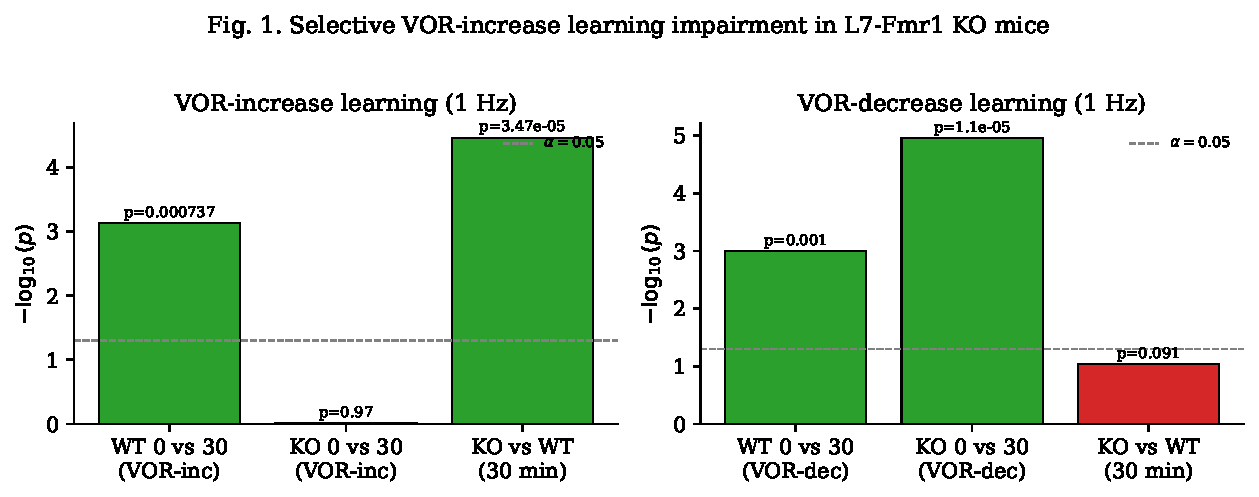
\includegraphics[width=0.95\textwidth]{figures/fig1_selective_impairment.pdf}
\caption{\textbf{Selective VOR-increase learning impairment in L7-Fmr1 KO mice.}
Bars show $-\log_{10}$ of the Tukey post-hoc $p$-values extracted from the
VOR experiments with 1 Hz sinusoidal vestibular-visual pairing.
Green bars indicate $p < 0.05$ (significant difference), red bars indicate
not-significant. WT mice learned both the VOR-increase
($p=7.37\times10^{-4}$, 0 vs 30 min) and VOR-decrease ($p=0.001$) tasks;
L7-Fmr1 KO mice failed on VOR-increase ($p=0.97$; KO vs WT
$p=3.47\times10^{-5}$) but learned VOR-decrease normally
($p=1.10\times10^{-5}$; KO vs WT $p=0.091$).}
\label{fig:selective_impairment}
\end{figure}

\begin{figure}[htbp]
\centering
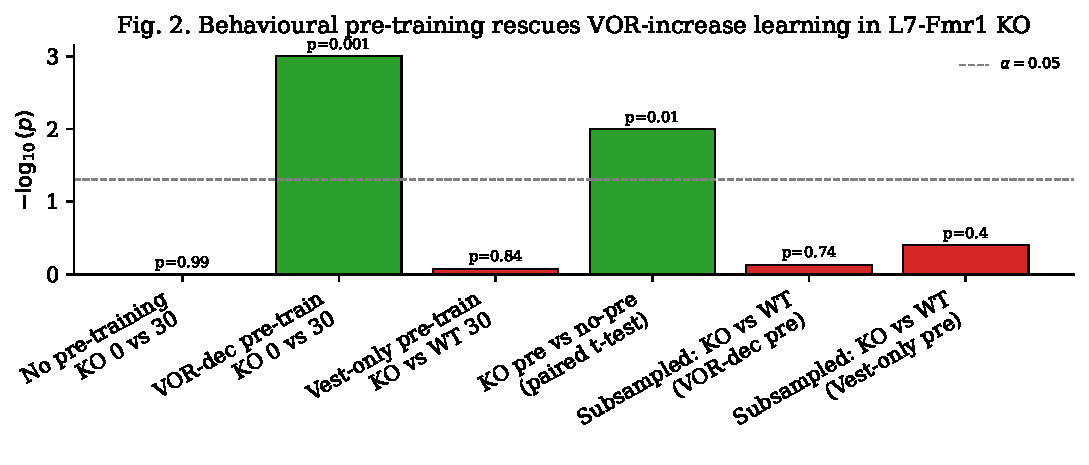
\includegraphics[width=0.95\textwidth]{figures/fig2_behavioral_pretraining.pdf}
\caption{\textbf{Behavioural pre-training rescues VOR-increase learning in
L7-Fmr1 KO mice.} Extracted Tukey or paired $t$-test $p$-values. Without
pre-training, KO animals did not learn ($p=0.99$, 0 vs 30 min); after
30 min of VOR-decrease pre-training, they did ($p=0.001$). Vestibular-only
pre-training produced a KO vs WT comparison of $p=0.84$. The within-mouse
comparison (no-pre vs pre) was $p=0.01$ in the KO cohort. Subsampling for
matched pre-training-induced decreases preserved the rescue.}
\label{fig:behavioral_pretraining}
\end{figure}

\begin{figure}[htbp]
\centering
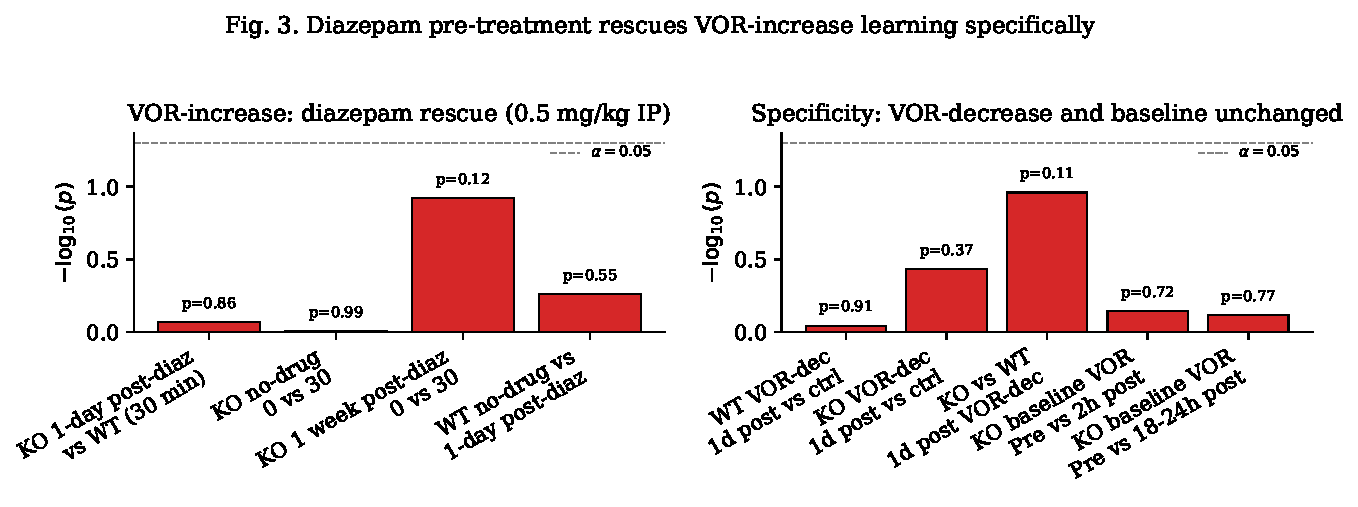
\includegraphics[width=0.95\textwidth]{figures/fig3_diazepam_rescue.pdf}
\caption{\textbf{Diazepam pre-treatment (0.5 mg/kg IP, 18--24 h prior)
rescues VOR-increase learning specifically.} Left, rescue of the 1-Hz
VOR-increase learning deficit (KO vs WT at 30 min post-diazepam $p=0.86$);
the rescue is absent 1 week later ($p=0.12$, 0 vs 30 min). Right, specificity:
VOR-decrease learning and baseline VOR gain are unchanged by the drug in
either genotype (WT $p=0.91$; KO $p=0.37$; KO vs WT $p=0.11$; baseline
gains $p \geq 0.36$).}
\label{fig:diazepam_rescue}
\end{figure}

\begin{figure}[htbp]
\centering
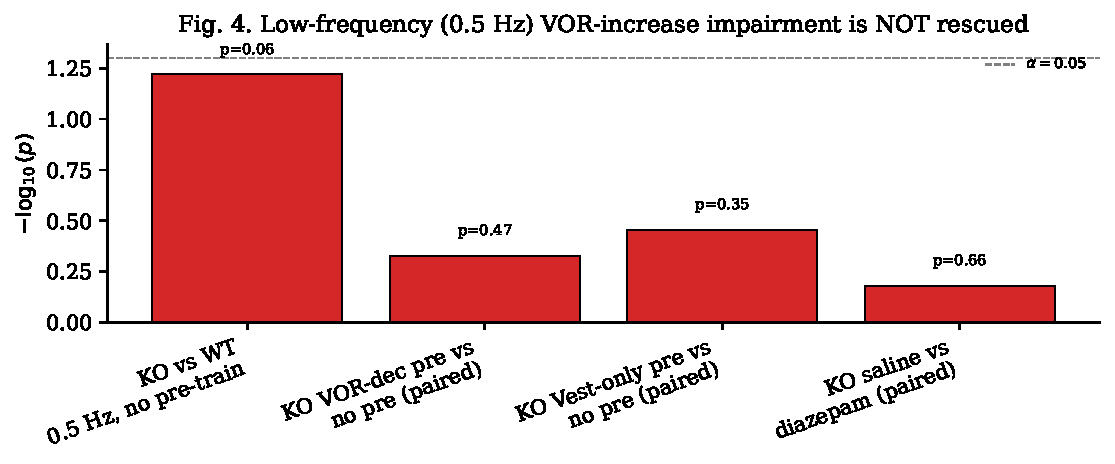
\includegraphics[width=0.95\textwidth]{figures/fig4_low_freq_no_rescue.pdf}
\caption{\textbf{Low-frequency (0.5 Hz) VOR-increase impairment is \emph{not}
rescued by behavioural pre-training or diazepam.} KO mice show a trend
toward impairment at 0.5 Hz ($p=0.06$ vs WT). Neither VOR-decrease
pre-training ($p=0.47$), vestibular-only pre-training ($p=0.35$), nor
diazepam pre-treatment ($p=0.66$) reversed it. This dissociation matches
prior evidence that PF--Purkinje-cell LTD contributes selectively to
high-frequency but not low-frequency VOR adaptation.}
\label{fig:low_freq_no_rescue}
\end{figure}

\begin{figure}[htbp]
\centering
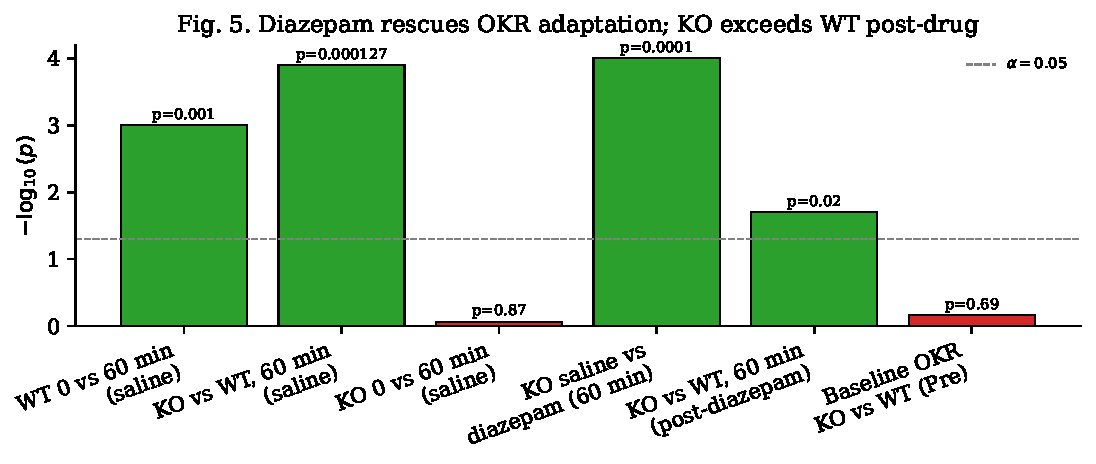
\includegraphics[width=0.95\textwidth]{figures/fig5_okr_rescue.pdf}
\caption{\textbf{OKR adaptation is rescued by diazepam, and post-drug KO
learning exceeds WT.} WT mice acquire the OKR adaptation over 60 min
($p=0.001$). KO mice fail post-saline ($p=0.87$, 0 vs 60 min; KO vs WT
$p=1.27\times10^{-4}$). 18--24 h post-diazepam, KO learning is rescued
(KO saline vs diazepam $p=0.0001$) and exceeds WT (KO vs WT $p=0.02$).
Baseline OKR gain is unaffected ($p=0.69$).}
\label{fig:okr_rescue}
\end{figure}

\begin{figure}[htbp]
\centering
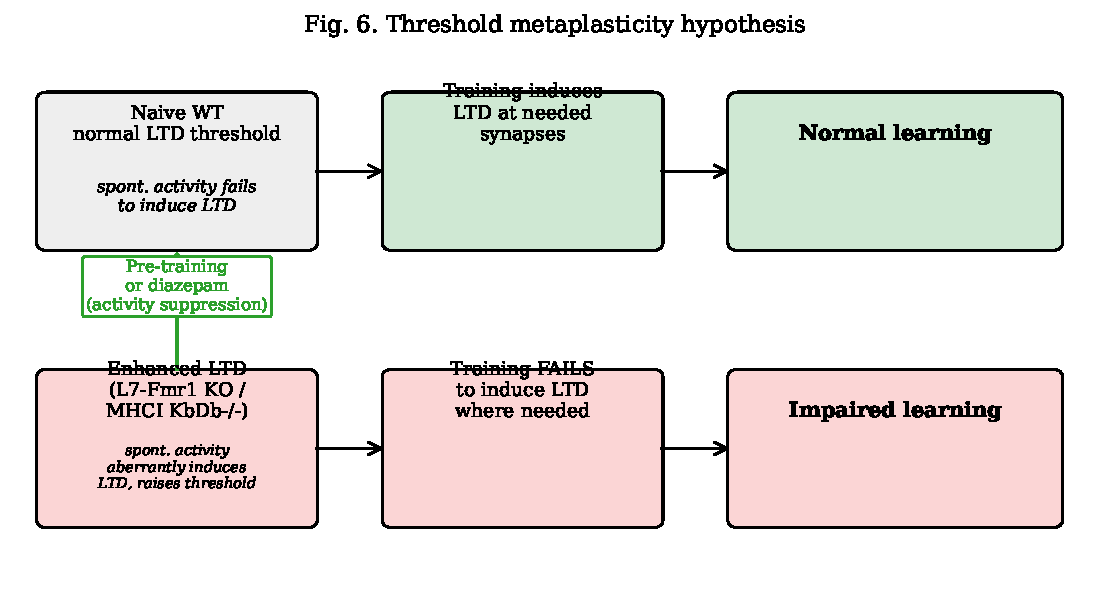
\includegraphics[width=0.85\textwidth]{figures/fig6_metaplasticity_schematic.pdf}
\caption{\textbf{Threshold metaplasticity hypothesis.} In naive WT mice the
threshold for associative PF--Purkinje-cell LTD is normal, so spontaneous
circuit activity does not aberrantly induce LTD, and training can recruit
LTD at the synapses where it supports learning. In L7-Fmr1 KO and
MHCI KbDb\textsuperscript{-/-} mice, enhanced LTD lowers the induction threshold,
allowing spontaneous activity to recruit LTD before training and thereby
raise the threshold for subsequent induction --- leaving LTD unavailable
to support learning during training. Pre-training or diazepam suppresses
activity-driven induction before training and resets the threshold,
restoring LTD-dependent learning.}
\label{fig:metaplasticity}
\end{figure}
